\section{Experiments}
\label{sec:experiments}
In this section we report on the experimental evaluation and comparison of the click models in Section~\ref{sec:methodology} on the evaluation metrics in Section~\ref{sec:evaluation} evaluated on the first 1 million query sessions from the Yandex Relevance Prediction contest of 2011 \cite{YandexData}. The rest of this section will elaborate on the experiments we have done and the results we found. We will also show how query frequency improves the performance of the models. Moreover, we will report on the evaluation measures in combination with click entropy.

\subsection{Experimental Setup}
The Yandex data set was used in the Yandex Relevance Prediction contest of 2011. In the experiments we have done we have used the first 1 million queries. We deliberately have chosen to keep sessions that are without any clicks because removing them might hurt the performance of certain models, i.e. TCM because the freshness of a document can change with these sessions. These first 1 million sessions contain 450,931 distinct queries. These queries get divided into a set of training sessions used to train the click models and a set of test sessions used in the evaluation of the models, the number of sessions in these sets have a 3 to 1 ratio. The problem with this approach in combination with the TCM model is that this removes the guarantee that the complete task is used when training or evaluating the model. We expect that this will hurt the performance of the TCM model and that the actual performance might be higher. 

\subsubsection{Performance impacting factors}
To report on the performance with regard to query frequency we have split the data into 4 parts. The distribution of these parts can be seen in Table~\ref{table:query_split}.We see that there are a lot of queries that are only seen once, these queries are not informative for the models that only look at relevance, e.g. the CTR and CM models, however they are informative for the other models to infer other parameters than relevance. We also see that there are few queries In the rest of this section with every evaluation measure we will also report on how this was influenced by the query frequency. We did this by only using the sessions for a particular group of query frequencies. This way all parameters can be optimal for these frequencies. This does raise a problem however for the query frequency bin of 6 to 19, here there are so few queries it is hard for the models to learn the correct parameters. This will have a negative effect on the performance of the models. 

The second factor that might influence performance that we have analyzed is the click entropy. The click entropy was also used to analyze queries in \cite{dou2008}.The formal definition is shown in Equation~\ref{eq:entropy}.

\begin{align}
	ClickEntropy(q) &= \sum_{d \in \mathcal{P}(q)} - P(d|q) \log_2 P(d|q) \label{eq:entropy} \\
	P(d|q) &= \frac{\sum_p c_{r_d}^{(q)}}{\sum_{u \in \mathcal{P}(q)} c_{r_u}^{(q)}} \label{eq:entropy_2}
\end{align}

Here $ClickEntropy(q)$ is the click entropy for query $q$. $\mathcal{P}(q)$ are documents clicked on when regarding query $q$. $P(d|q)$ is the percentage of clicks on document $d$ among all clicks on $q$.  Click entropy can be used to split the data into informational and navigational queries. In navigational queries users know what they are looking for so the click entropy will be low because almost all clicks within that query will be on the same document. In a informational query the users explore different results to find the optimal one because they don't know what document they are looking for yet. This will give these queries a high click entropy.
The search sessions have been divided into 3 parts with respect to click entropy and the evaluation measures have been tested on these parts in the same way as query frequency. Statistics of these parts can be seen in Table~\ref{table:entropy_split}.
\\

\begin{minipage}[b]{.45\textwidth}
	\centering
\begin{tabular}{lc}
\hline
Query frequency & Number of sessions \\ \midrule
1               & 392508            \\ 
2 - 5           & 123799            \\ 
6 - 19          & 63596             \\ 
20 +            & 420097            \\ \bottomrule
\end{tabular}
\captionof{table}{The distribution of session with respect to query frequency}
\label{table:query_split}
\end{minipage}
\qquad
\begin{minipage}[b]{.45\textwidth}
	\centering
\begin{tabular}{lc}
\toprule
Click entropy & Number of sessions \\ \midrule
0 - 1         & 509062             \\ 
1+ - 2        & 154672             \\ 
2+            & 336266             \\ \bottomrule \\
\end{tabular}
\captionof{table}{The distribution of session with respect to click entropy}
\label{table:entropy_split}
\end{minipage}

\subsection{Results}
In this section we outline the results of the experiments. For every evaluation measure the influence of the query frequency and click entropy can be seen. Table~\ref{table:results} contains the values of the evaluation measures for every model when trained on the entire dataset.

\subsubsection{Loglikelihood}
In Figures \ref{fig:ll_qf} and \ref{fig:ll_ce} the results of the loglikelihood experiments can be seen. We want the loglikelihood to be as close to 0 as possible. The loglikelihood of the Cascade Model is not measured as the likelihood of a session with multiple clicks is undefined for that model. We see that UBM is the model that performs best when training on the whole data set and only on the queries with average click-entropy, between 1 and 2, the model is outperformed by CCM. We expected UBM to be the best model going into these experiments. Something to note is that the PBM performs well on queries that have low entropy, a sign that the examination parameters are more accurate on informational queries.

An interesting thing to see is that the loglikelihood gets more negative when looking at the queries with 20+ sessions. We think this is because queries that happen more frequently will also have more documents that are shown to the user overall. This means that a particular document is shown less to the model which makes it harder to predict the click probability.

\begin{figure}
	\centering
	\begin{subfigure}[b]{.49\textwidth}
	\centering
		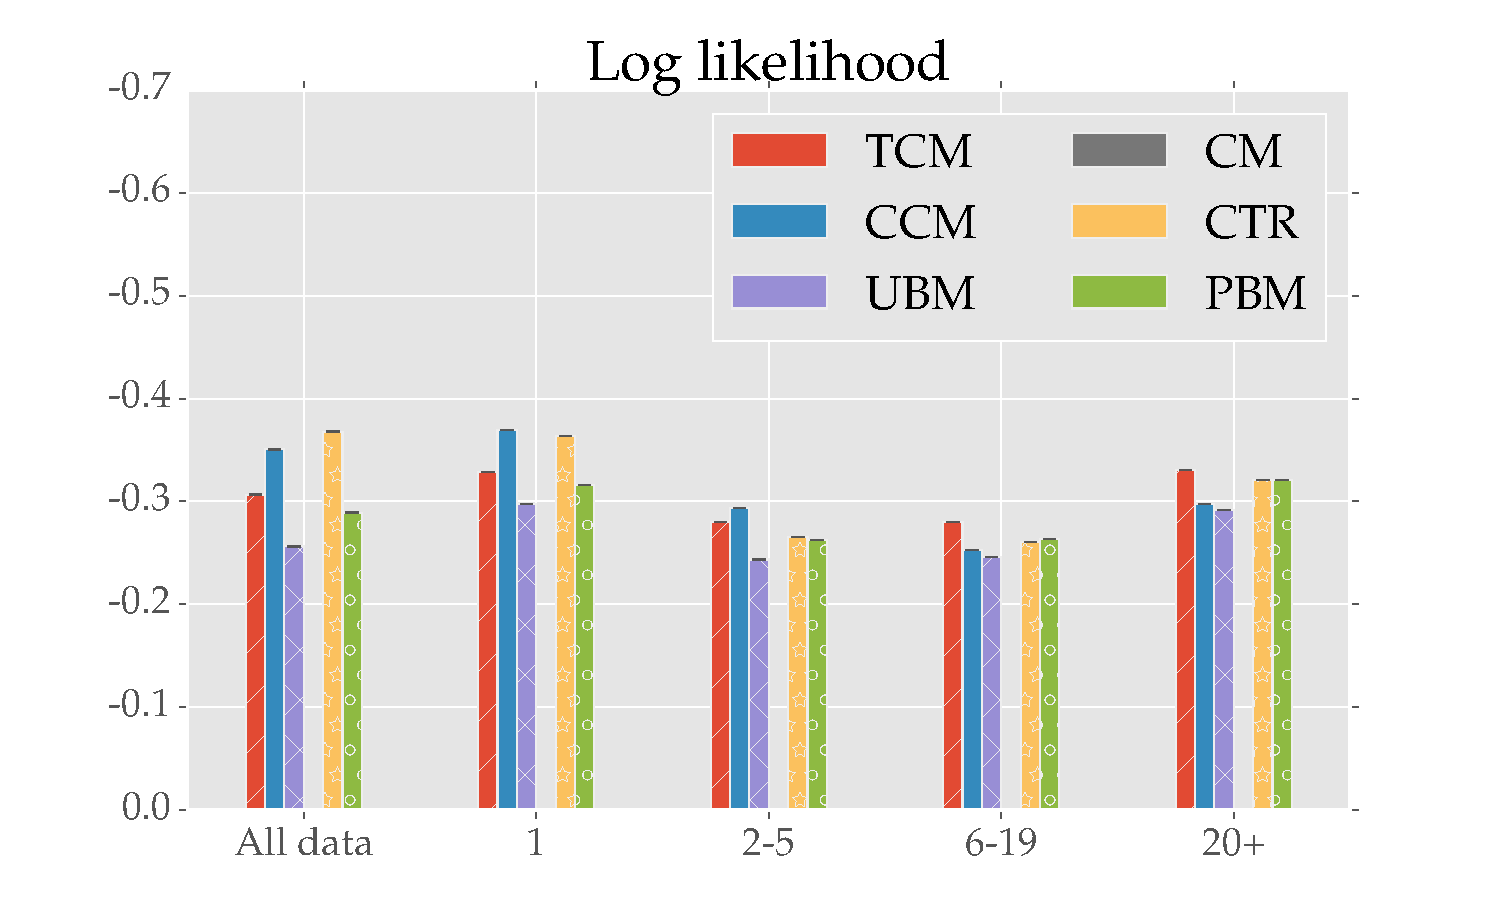
\includegraphics[width=\textwidth]{figures/LL_qf.pdf}
		\caption{Query frequency}
		\label{fig:ll_qf}
	\end{subfigure}
	\begin{subfigure}[b]{.49\textwidth}
		\centering
		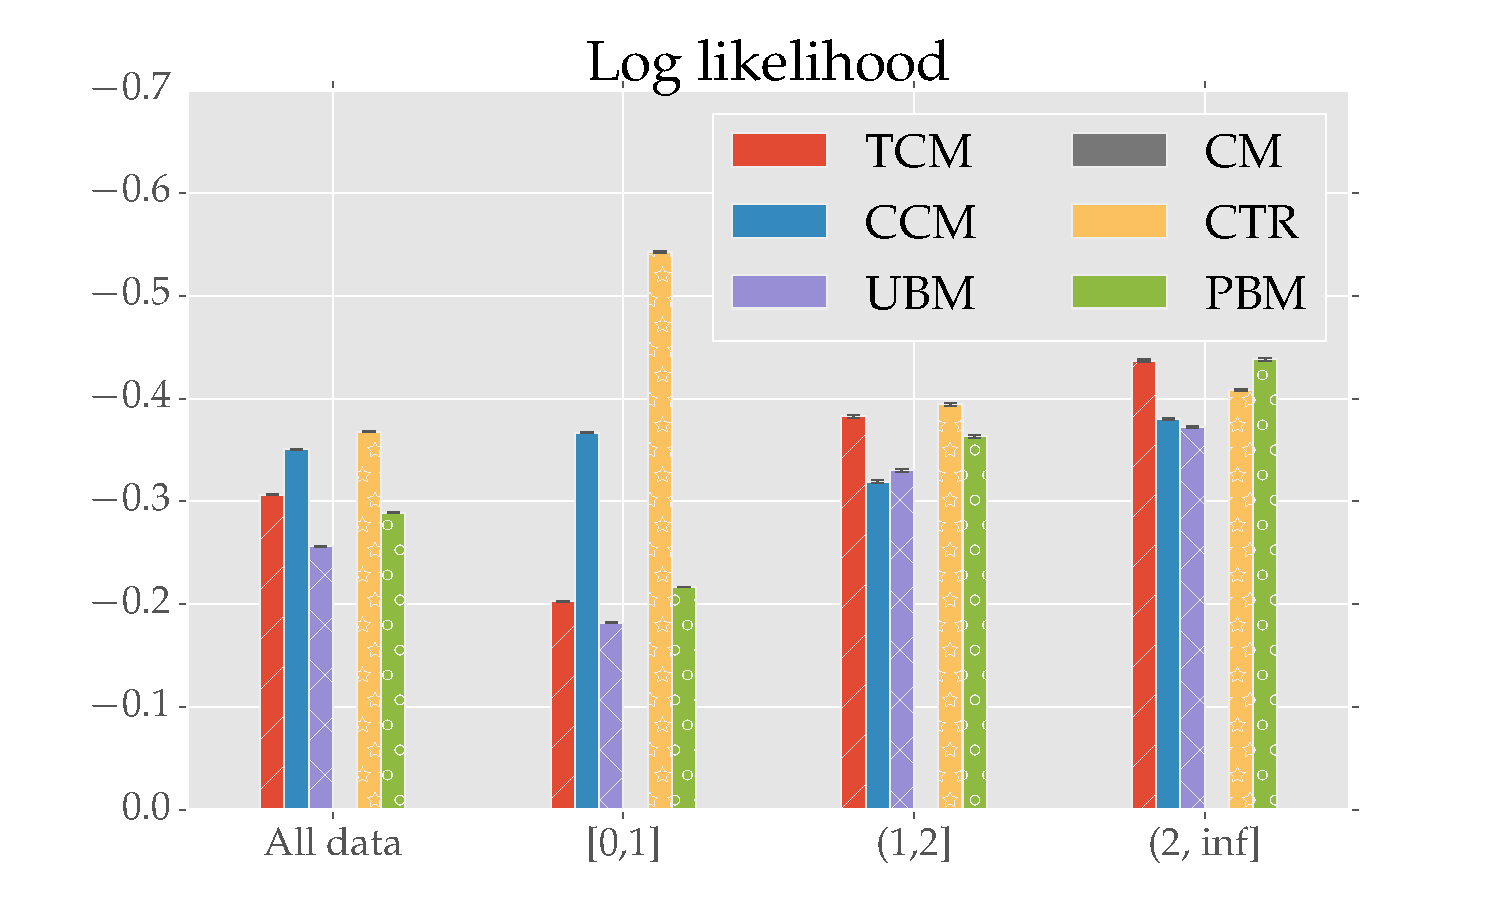
\includegraphics[width=\textwidth]{figures/LL_ce.pdf}
		\caption{Click entropy}
		\label{fig:ll_ce}
	\end{subfigure}
	\caption{Loglikelihood of click models}
\end{figure}


\subsubsection{Perplexity}
In Figures~\ref{fig:perp_qf} and \ref{fig:perp_ce} the influence of the query frequency and click entropy on the perplexity can be seen. The fact that TCM and PBM perform better than UBM is surprising considering the results of the loglikelihood-experiments. When we compare the figures of loglikelihood (\ref{fig:ll_qf},~\ref{fig:ll_ce}) and perplexity(\ref{fig:perp_qf},~\ref{fig:perp_ce}) with eachother we can see that UBM performs best on loglikelihood while not being the best on perplexity. This is due to the fact that the loglikelihood is the conditional probability of a click, seen in Equation~\ref{eq:loglikelihood} while perplexity uses the unconditional probabilities, seen in Equation~\ref{eq:perp_prob}. UBM uses the distance between the current document and the last click to determine the examination probability which is of course easier to compute if the last click is observed instead of marginalizing over all possible distances since the last click.

In Figure~\ref{fig:perp_rank} the perplexity of different ranks can be seen. As a document has a higher rank the models perplexity gets lower. However speed with which it gets lower differs per model. TCM and PBM have a high perplexity for the lower ranks, the documents that are more often examined by the users. Whereas for high ranks they are the top performers in terms of perplexity. What this shows is that position based click models, of which our implementation of TCM is one, the examination parameter is more accurate than the examination parameter inferred by other models.

\begin{figure}
	\centering
	\begin{subfigure}[b]{.49\textwidth}
		\centering
		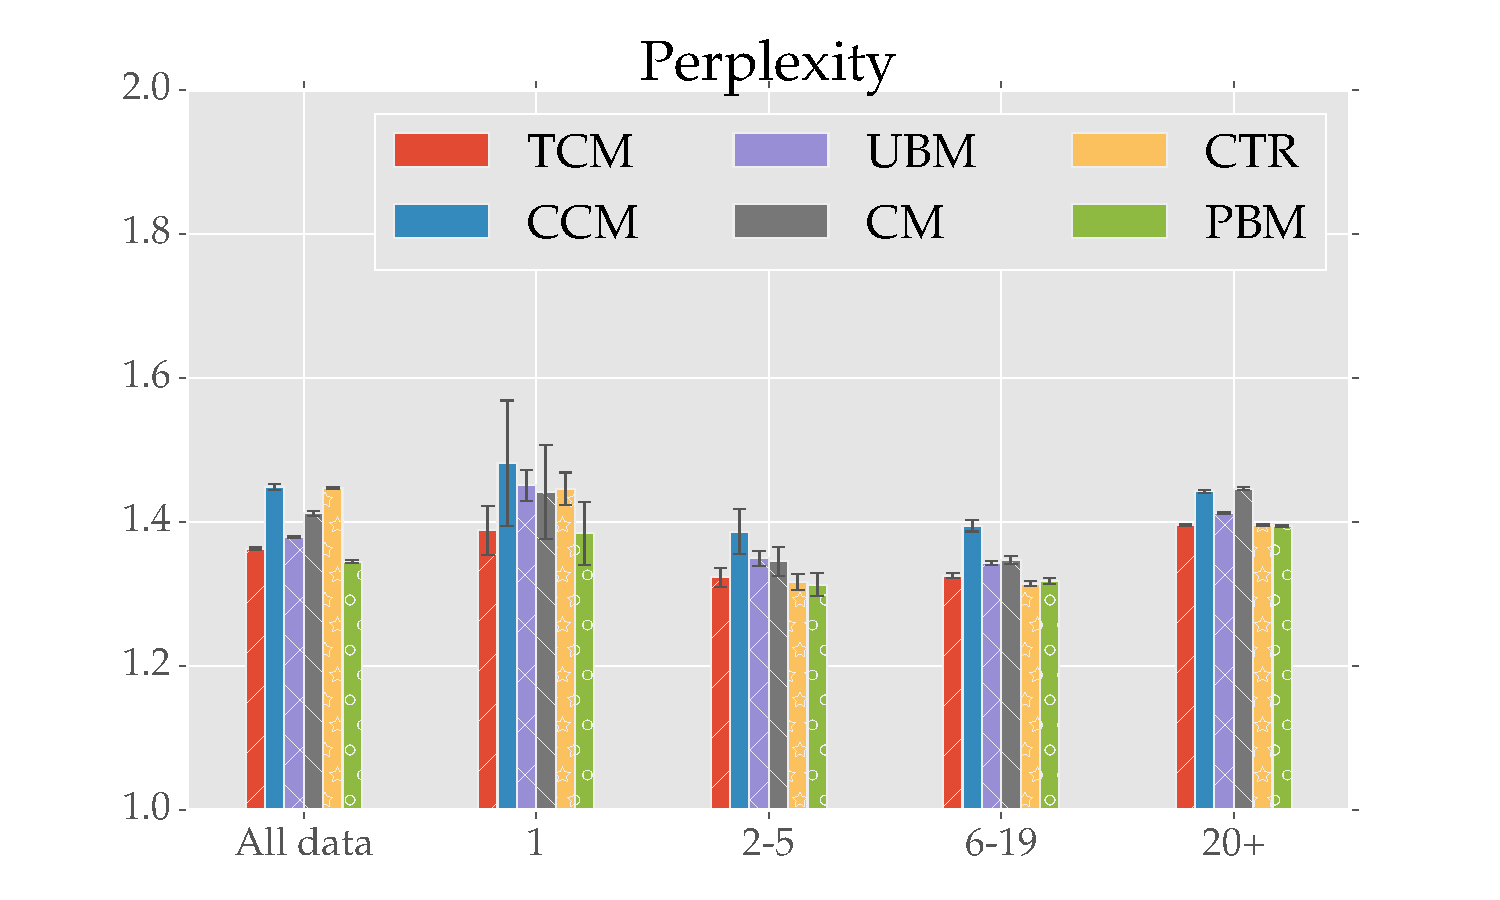
\includegraphics[width=\textwidth]{figures/Perp_qf.pdf}
		\caption{Query frequency}
		\label{fig:perp_qf}
	\end{subfigure}
	\begin{subfigure}[b]{.49\textwidth}
		\centering
		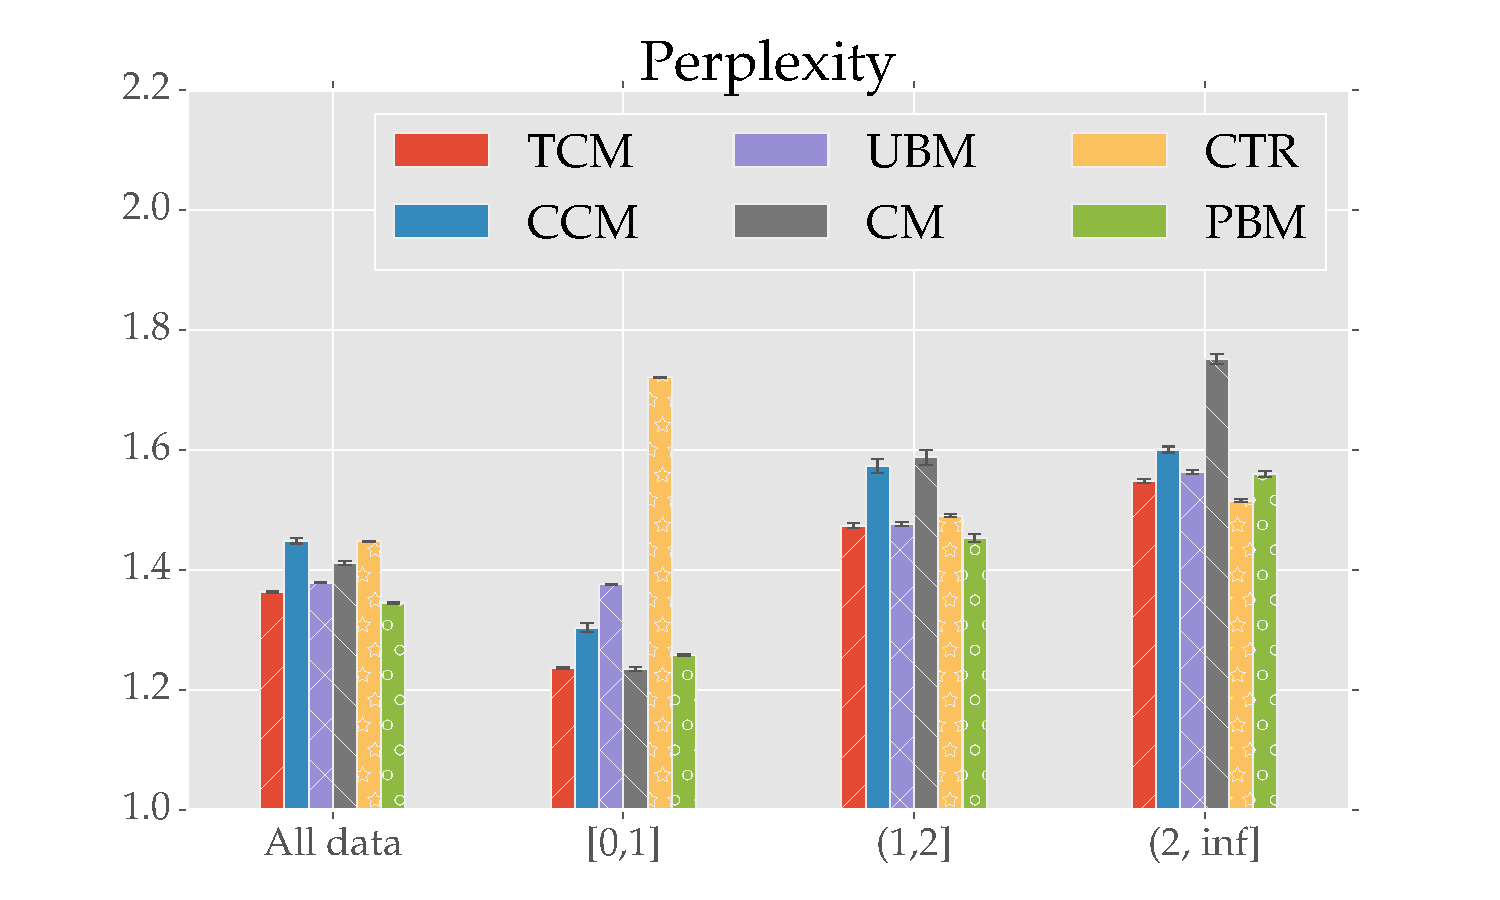
\includegraphics[width=\textwidth]{figures/Perp_ce.pdf}
		\caption{Click entropy}
		\label{fig:perp_ce}
	\end{subfigure}
	\caption{Perplexity of click models}
\end{figure}

\begin{figure}
	\centering
	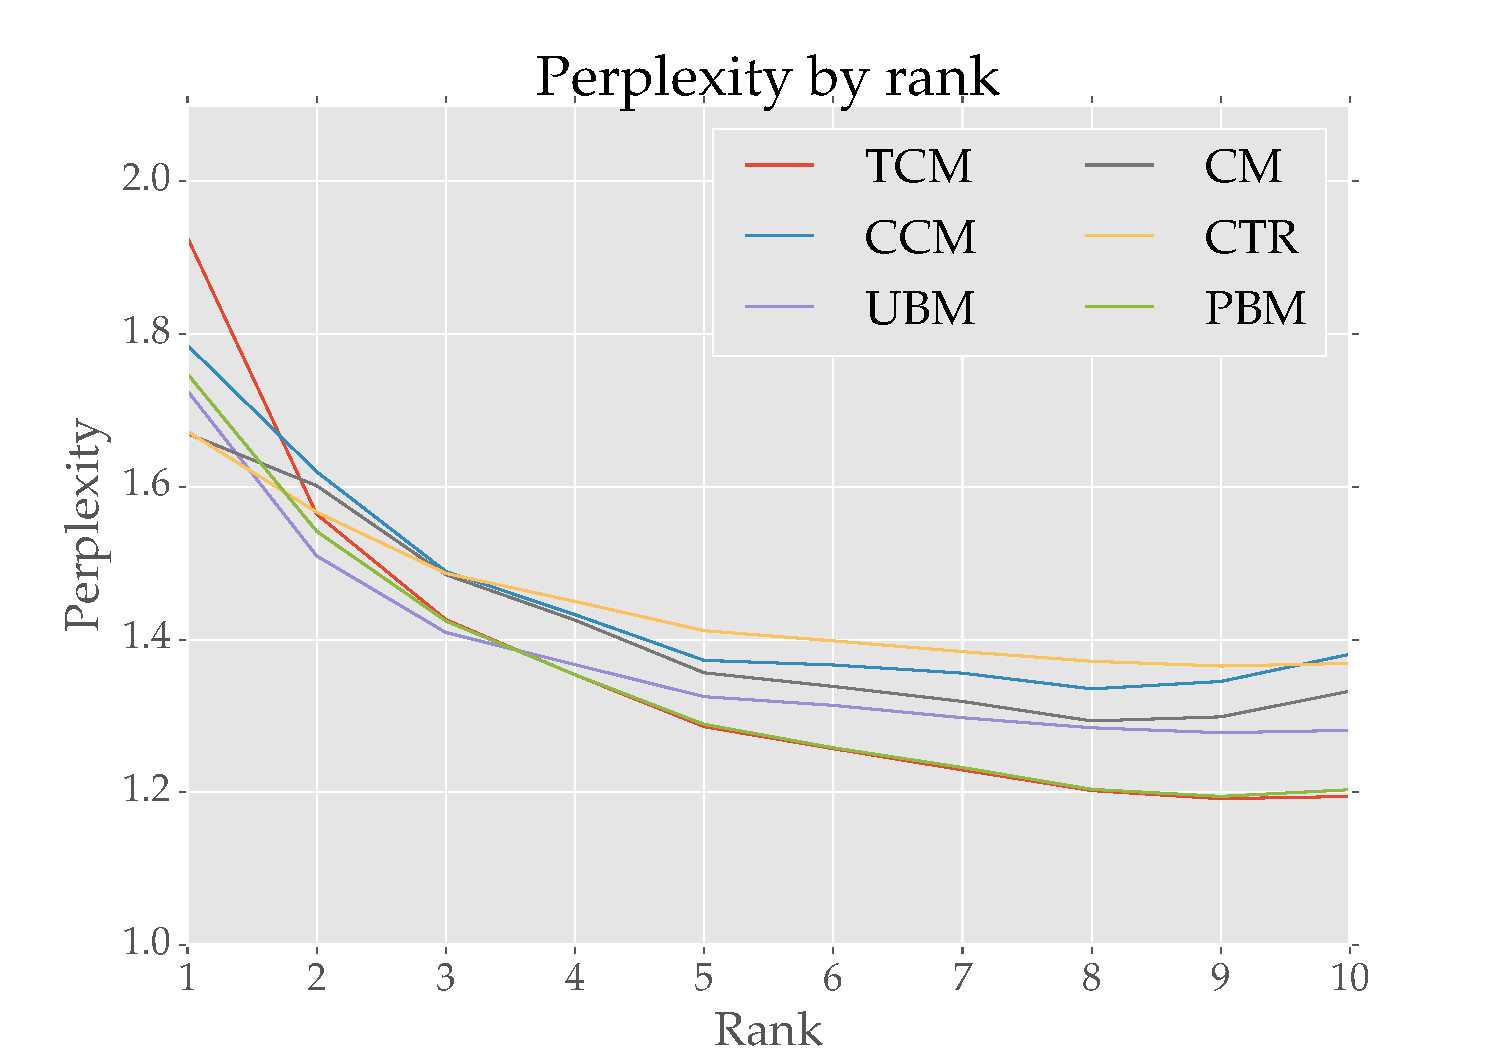
\includegraphics[width=.8\textwidth]{figures/Perp_rank.pdf}
	\caption{Perplexity of click models at different document rank position}
	\label{fig:perp_rank}
\end{figure}


\subsubsection{CTR-Prediction}
Figures~\ref{fig:ctr_qf} and \ref{fig:ctr_ce} show the impact of query frequency and click entropy on the CTR-prediction task. In this task the simple models, CTR and CM, outperform the more complex ones. This is because the intuition of these models is exactly what this task has set out to measure. As seen in the explanation of this task in Section~\ref{sec:ctr} this task is designed to take away the position bias by only testing on the sessions where the document appears in the first place. However it is disappointing that the complex models perform so much worse. This may have to do with the fact that every time the models are trained on a very small sample of the entire dataset. A consequence of this is that the other parameters, that are used by the complex models besides the relevance parameter, have little data to train on which influences the relevance parameter. Because of this we propose to change the method for calculating the CTR-prediction. By not training on one query at a time but on all queries in the same time the other parameters will train better and thus models that use EM-inference have a better chance to learn the actual relevance of a document.

\begin{figure}
	\centering
	\begin{subfigure}[b]{.49\textwidth}
		\centering
		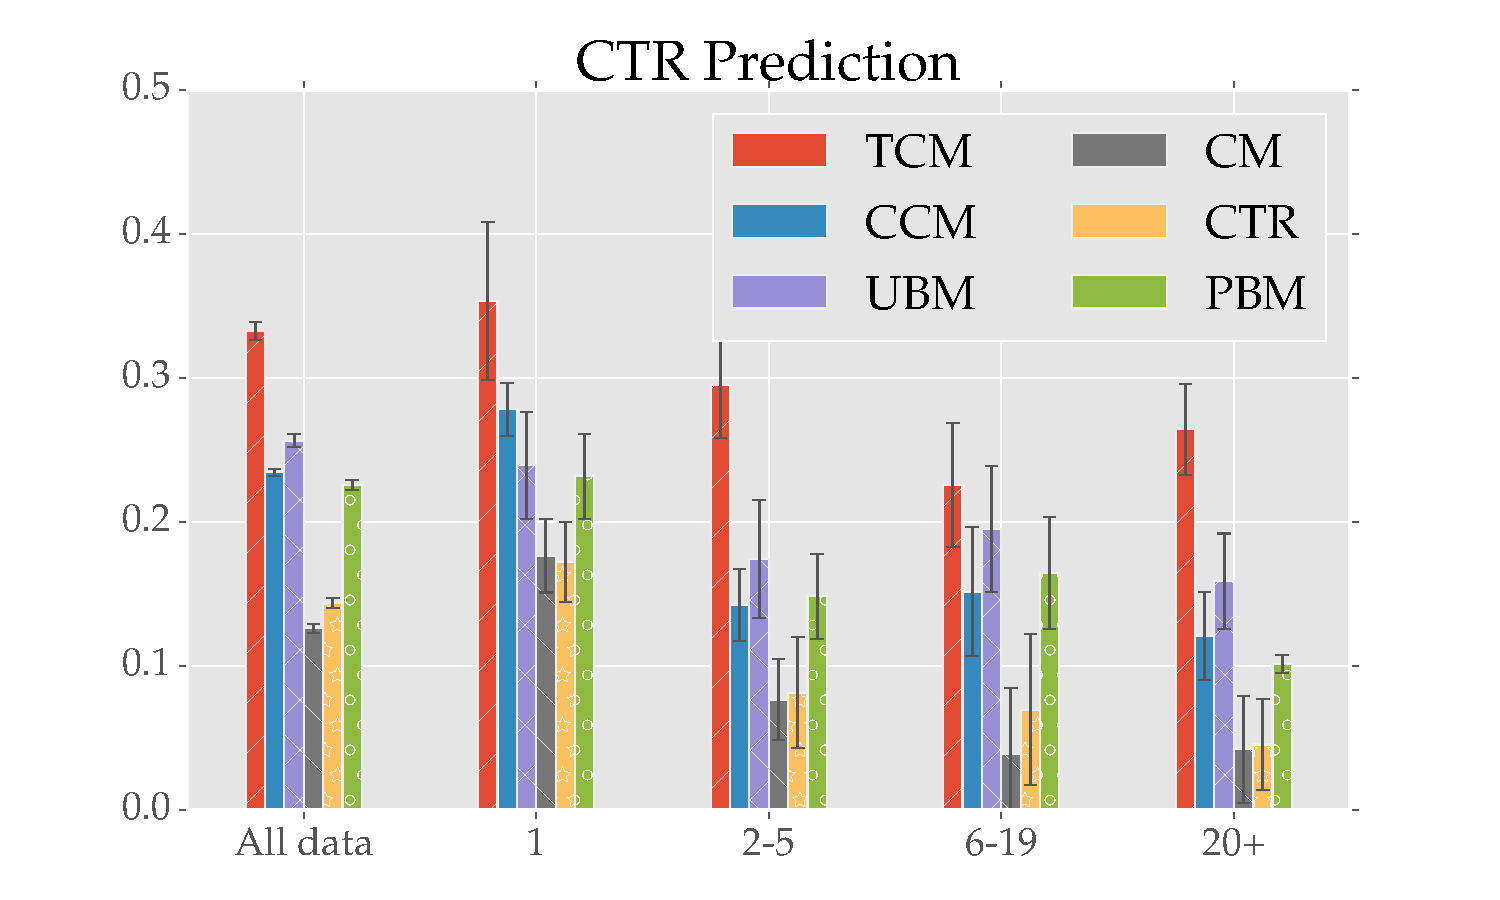
\includegraphics[width=\textwidth]{figures/CTRPred_qf.pdf}
		\caption{Query frequency}
		\label{fig:ctr_qf}
	\end{subfigure}
	\begin{subfigure}[b]{.49\textwidth}
		\centering
		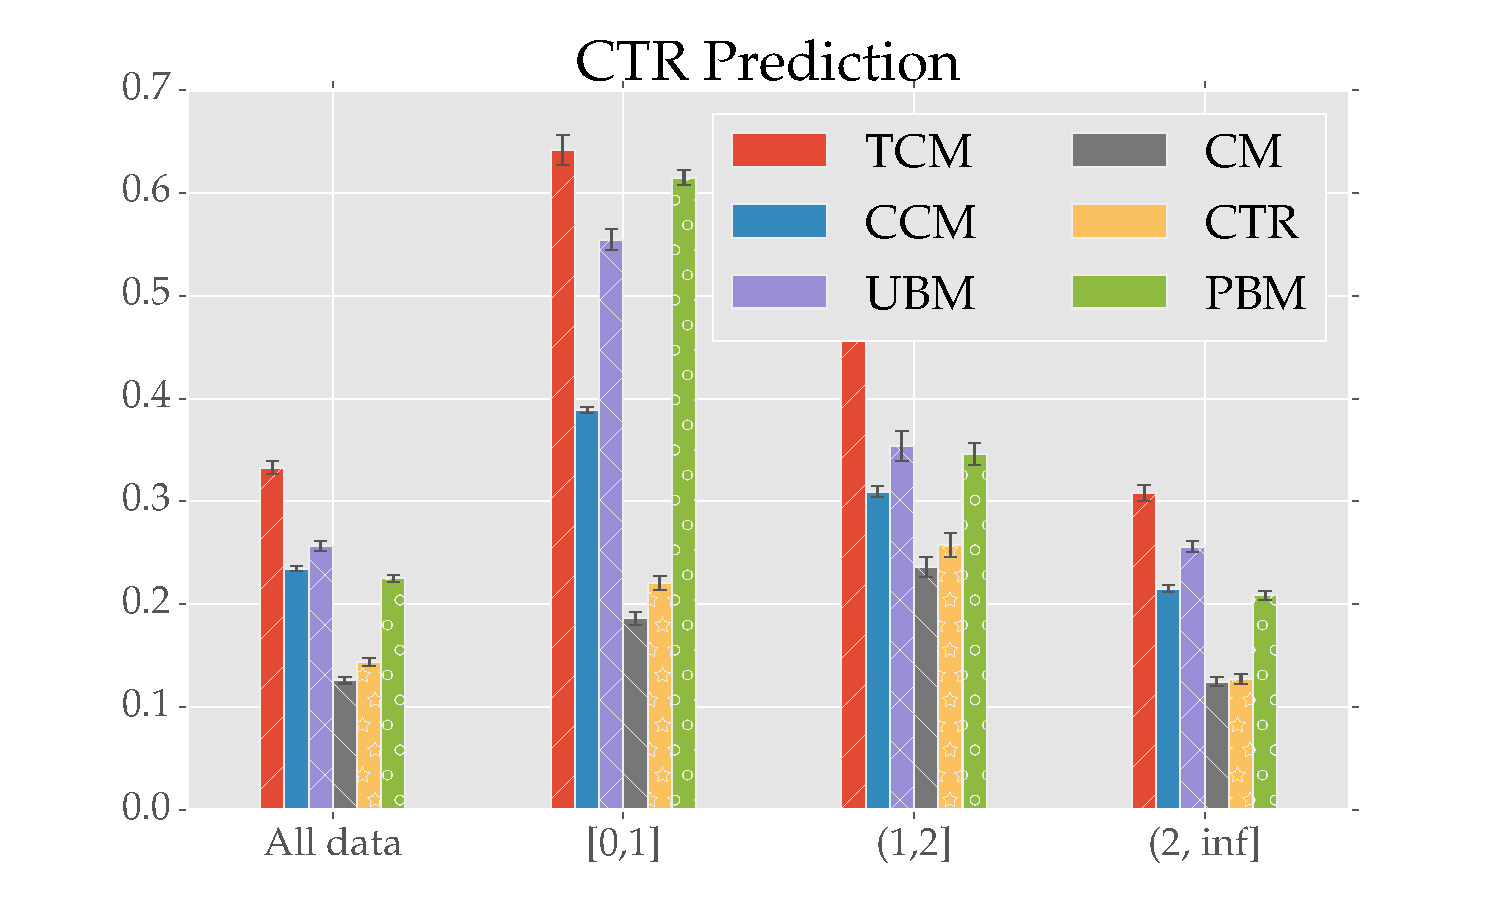
\includegraphics[width=\textwidth]{figures/CTRPred_ce.pdf}
		\caption{Click entropy}
		\label{fig:ctr_ce}
	\end{subfigure}
	\caption{Click-through rate of click models}
\end{figure}

\subsubsection{Relevance Prediction}
The results of the relevance prediction task can be seen in Figure~\ref{fig:rel_ce}. The plot for query frequency could not be generated for the lower query frequencies because the protocol for calculation only takes queries into account that occur more than 10 times. Even for the click entropy the results for the different splits are not as interesting as all models perform close almost the same. The models are trained only on the small subset of data and are evaluated on all query-document pairs found in the set of annotated relevances a lot of pairs are never seen before by the model. The model will then predict $0.5$, whereas the annotated relevance is always $0$ or $1$. This means that for all unseen query-document pairs the model will get a RMSE of 0.5 and the effect of document-query pairs that are seen will be negligible. When looking at the models that are trained on all the data we can see that the AUC gets lower then 0.5 this means that the predicted relevances have a negative correlation with the annotated relevances, which is illustrated by the Pearson correlation values we found. The values that were found there were between the 0.05 and -0.05, depending on whether the AUC was above or below 0.5. The p-values that we have found were all below 0.05 and indicate that the test is statiscally significant.

\begin{figure}
	\centering
	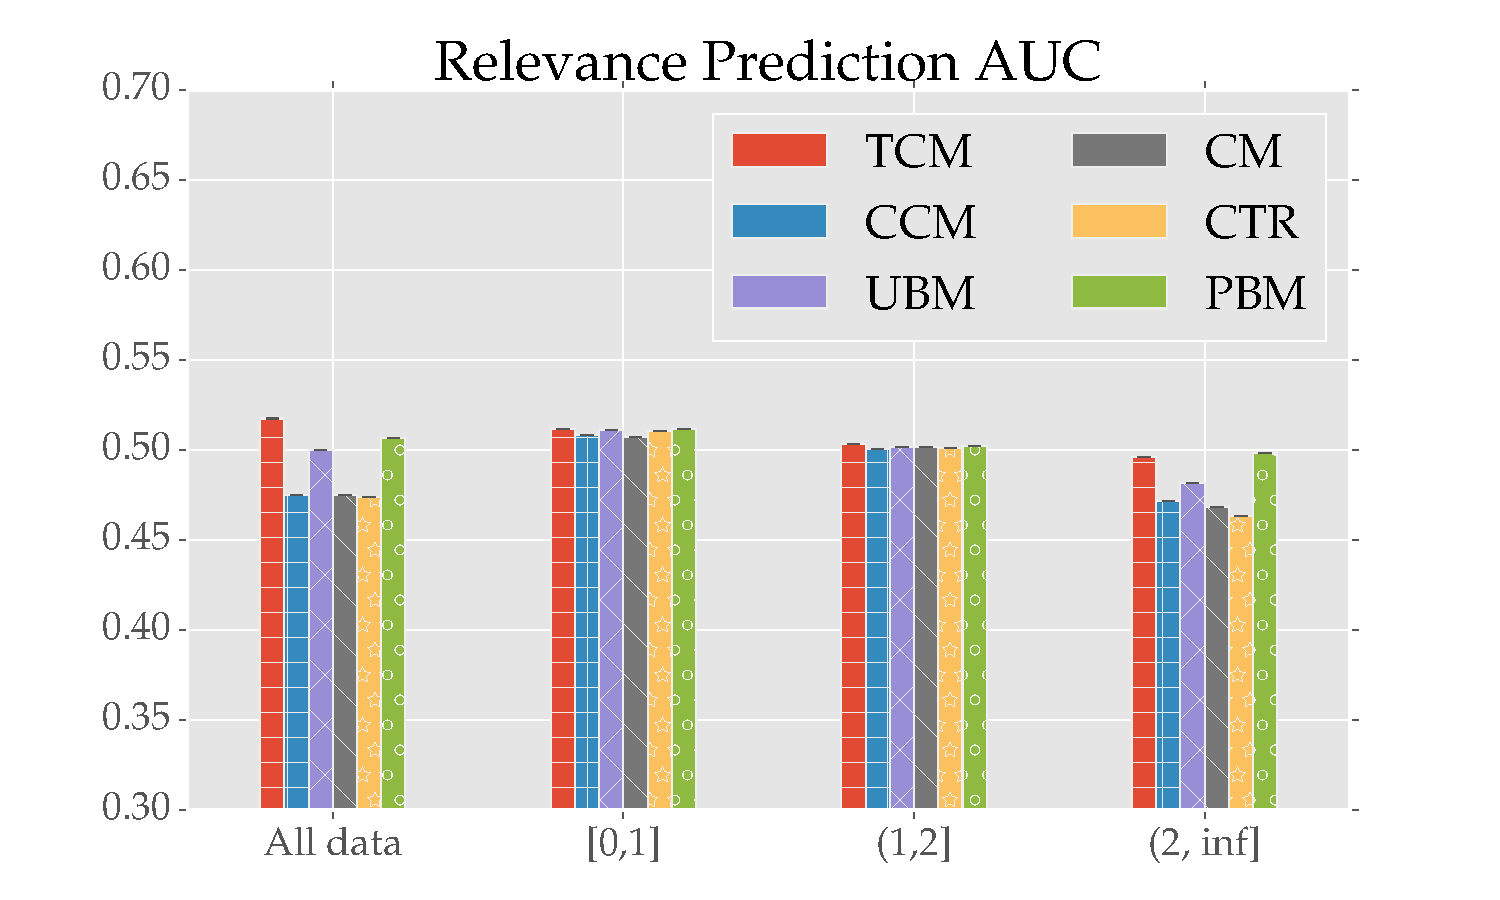
\includegraphics[width=.49\textwidth]{figures/Rel_Pred_AUC_ce.pdf}
	\caption{Relevance prediction of click models on click entropy}
	\label{fig:rel_ce}
\end{figure}

\subsubsection{Predicted Relevance as a Ranking Feature}
In Figures~\ref{fig:rank_qf} and~\ref{fig:rank_ce} the results of using the predicted relevance as a ranking feature can be seen. These results are not as good as expected, especially for the 6-19 query frequency bin. For the 6-19 query frequency bin the explanation for this performance is the fact that there are few queries for this bin. 

\begin{figure}
	\centering
	\begin{subfigure}[b]{.49\textwidth}
		\centering
		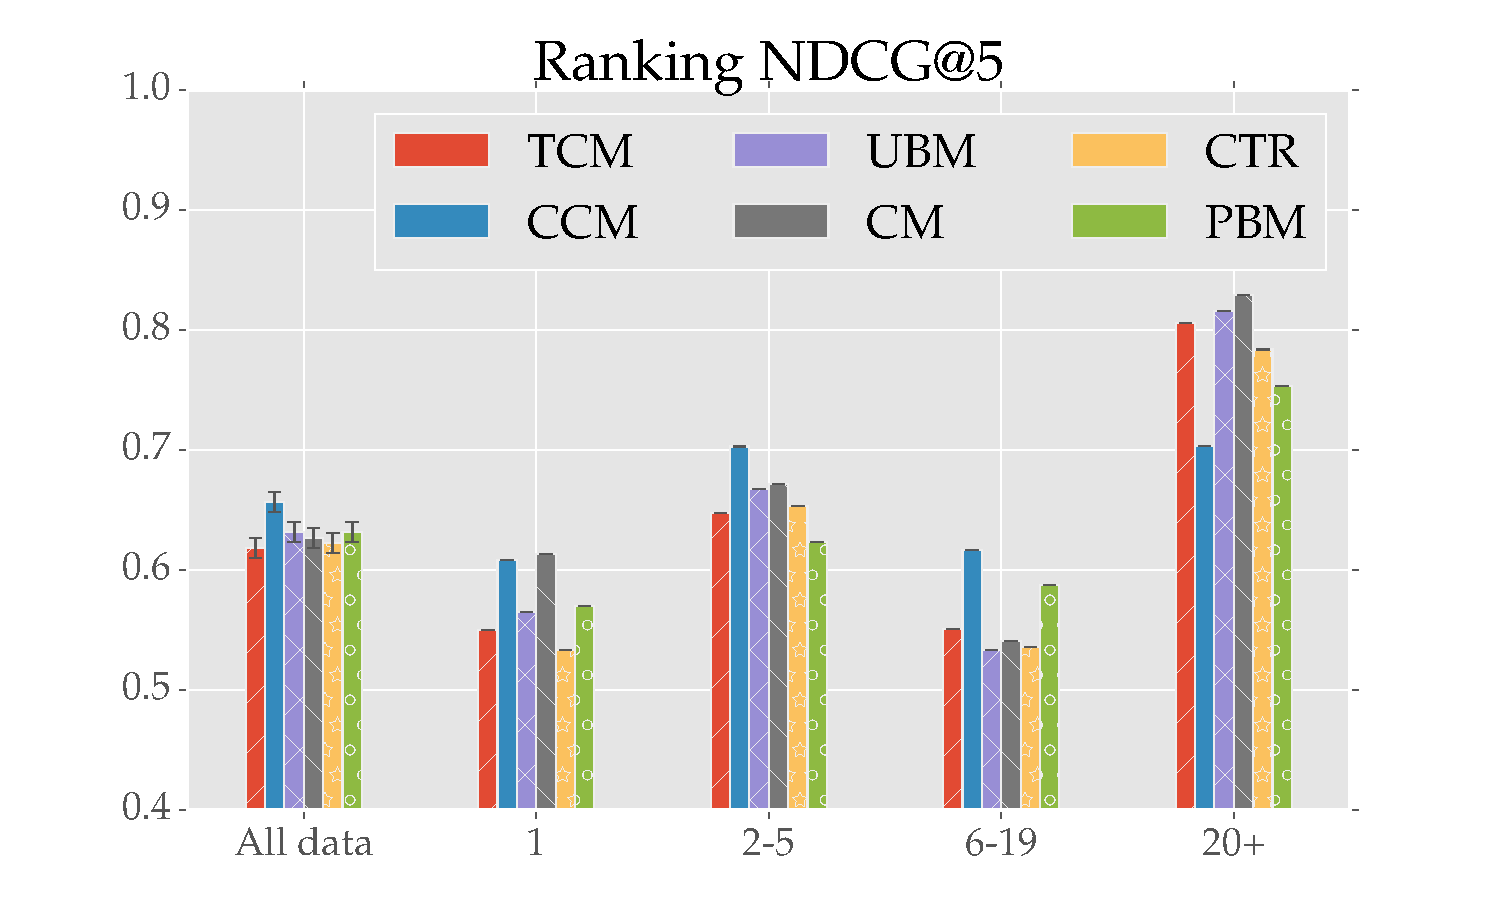
\includegraphics[width=\textwidth]{figures/Ranking_NDCG_qf.pdf}
		\caption{Query frequency}
		\label{fig:rank_qf}
	\end{subfigure}
	\begin{subfigure}[b]{.49\textwidth}
		\centering
		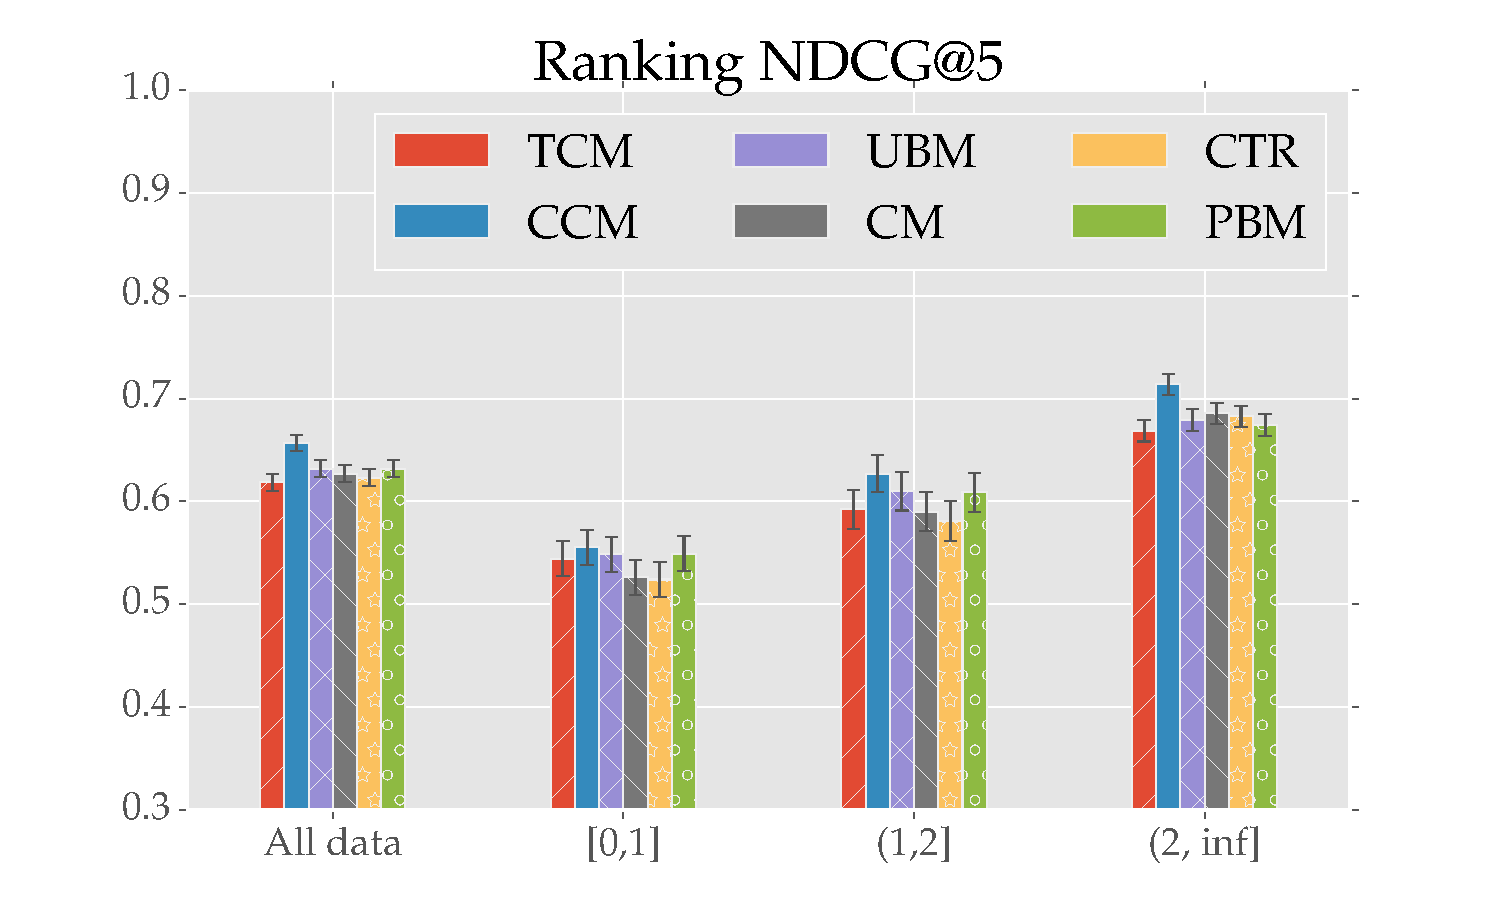
\includegraphics[width=\textwidth]{figures/Ranking_NDCG_ce.pdf}
		\caption{Click entropy}
		\label{fig:rank_ce}
	\end{subfigure}
	\caption{Ranking prediction of click models}
\end{figure}


\subsubsection{Computation time}
In Table~\ref{table:results} we see that, as expected, the models that use MLE-inference are much faster than the models with EM-inference. These training times depend on the number of queries that the model is trained upon and the amount of parameters a model has. An interesting thing to note is that the UBM model out performs TCM and CCM by a large margin.

\begin{table}
	\centering
	\begin{tabular}{lcccccccc}
		\toprule
		Model	&	Comp.Time.	&	$\mathcal{LL}$	&	Perp.	&	Rel.Pred.AUC	&	Rel.Pred.COR	&	Rel.Pred.Pval	&	Ranking	&	CTRPred. \\ \midrule
		TCM	&	8731.38	&	-0.307	&	1.363	&	0.518	&	0.0760	&	2.633e-52	&	0.619	&	0.333 \\
		CCM	&	10429.4	&	-0.3516	&	1.448	&	0.475	&	-0.0475	&	1.974e-21	&	0.657	&	0.234 \\
		UBM	&	5361.18	&	-0.256	&	1.379	&	0.5		&	0.0159	&	0.00149		&	0.632	&	0.257 \\
		CM	&	139.402	&	nan		&	1.412	&	0.475	&	-0.0607	&	6.712e-34	&	0.627	&	0.126 \\
		CTR	&	119.683	&	-0.368	&	1.448	&	0.474	&	-0.0529	&	3.762e-26	&	0.623	&	0.144 \\
		PBM	&	3897.65	&	-0.289	&	1.345	&	0.507	&	0.0361	&	5.518e-13	&	0.632	&	0.225 \\ \bottomrule \\
	\end{tabular}
	\caption{The results for the experiments on the first million sessions of the dataset. Comp.Time. is Computation time, $\mathcal{LL}$ is the loglikelihood. Perp. is the average perplexity over all ranks. Rel.Pred.AUC is the AUC of the relevance prediction task. Rel.Pred.COR and Rel.Pred.Pval are the Pearson correlation and p-value. Ranking is the NDCG@5 for the ranking performance and CTRPred. is the RMSE of the CTR-prediction task.}
	\label{table:results}
\end{table}

\subsubsection{Significance test}
To determine whether a result is statistically significant, we did a significance test for every session on every evaluation metric criteria. In this report we used two methods: two-tailed student-t test and standard error of the mean. For two-tailed student-t test, we use $\alpha = 0.05$ which commonly used to test the "null hypothesis". 

The standard error of the mean (SEM) is the standard deviation of the sample-mean's estimate of a population mean or can be formalize as following equation:
\begin{align*}
	\text{SE}_{\bar{x}} = \frac{stdev}{\sqrt{|\mathcal{S}|}}
\end{align*}

In all cases of our experiments, the p-value of student-t tests have a complete correlation with SEM.
Therefore, we only included the SEM as error-bar on each figures, where the two values are statistically significant if there is no intersection between their error-bars.
These error bars can also be seen as the confidence level of click models with respect to the evaluation measurement.